%%
%% Author: shoupu_wan
%% 8/22/18
%%

\chapter{Minimum containing window}\label{ch:minimumContainingWindow}

Out of all the coding questions I've worked on, `Minimum containing window' is one of a few that
is well defined but the solution space is huge to explore and optimize.
This little problem makes a good exercise for coding practice with a relatively straightforward
algorithm.
I'm going to demonstrate in near real production development environment, how I jump in with a
rough initial idea and out with a readable, modular, well-designed solution.

\section{Problem statement}\label{sec:problemStatement.min-window}

The problem is stated as follows:
\begin{quote}
    Given a string \code{S} and a string \code{T}, find the minimum window in \code{S} which will
    contain all the characters in \code{T}\@.
\end{quote}

\section{Outline of the algorithm}\label{sec:outlineOfTheAlgorithm.min-window}

We are talk about implementation of a greedy algorithm which runs in $O(M+N)$ time complexity,
where $M$ and $N$ are the lengths of the strings \code{T} and \code{S}, respectively.

The idea behind the algorithm has two parts:
\begin{enumerate}
    \item Find a containing window;
    \item Attempts to `push-and-squash' the containing window to the smallest.
\end{enumerate}

Once initialized, the containing window, while maintains the containment invariant, moves like a
caterpillar.
It wiggles itself forward starting from the tail.
Namely, it attempts to shrink the window by attempting to wrap the left most char well within the
body of the window and if this is not possible, it attempts to expand to the right until the end
of the string.

A useful data structure is an intermediate buffer to account for the character surplus,
\textit{e.g.},
those characters in string \code{S} that could be used but not used in between the start and end
of the containing window.
Other data structures that are useful may be maps for char account.
If properly implemented, the algorithm runs with linear time.

\begin{figure}[htb]
    \begin{center}
        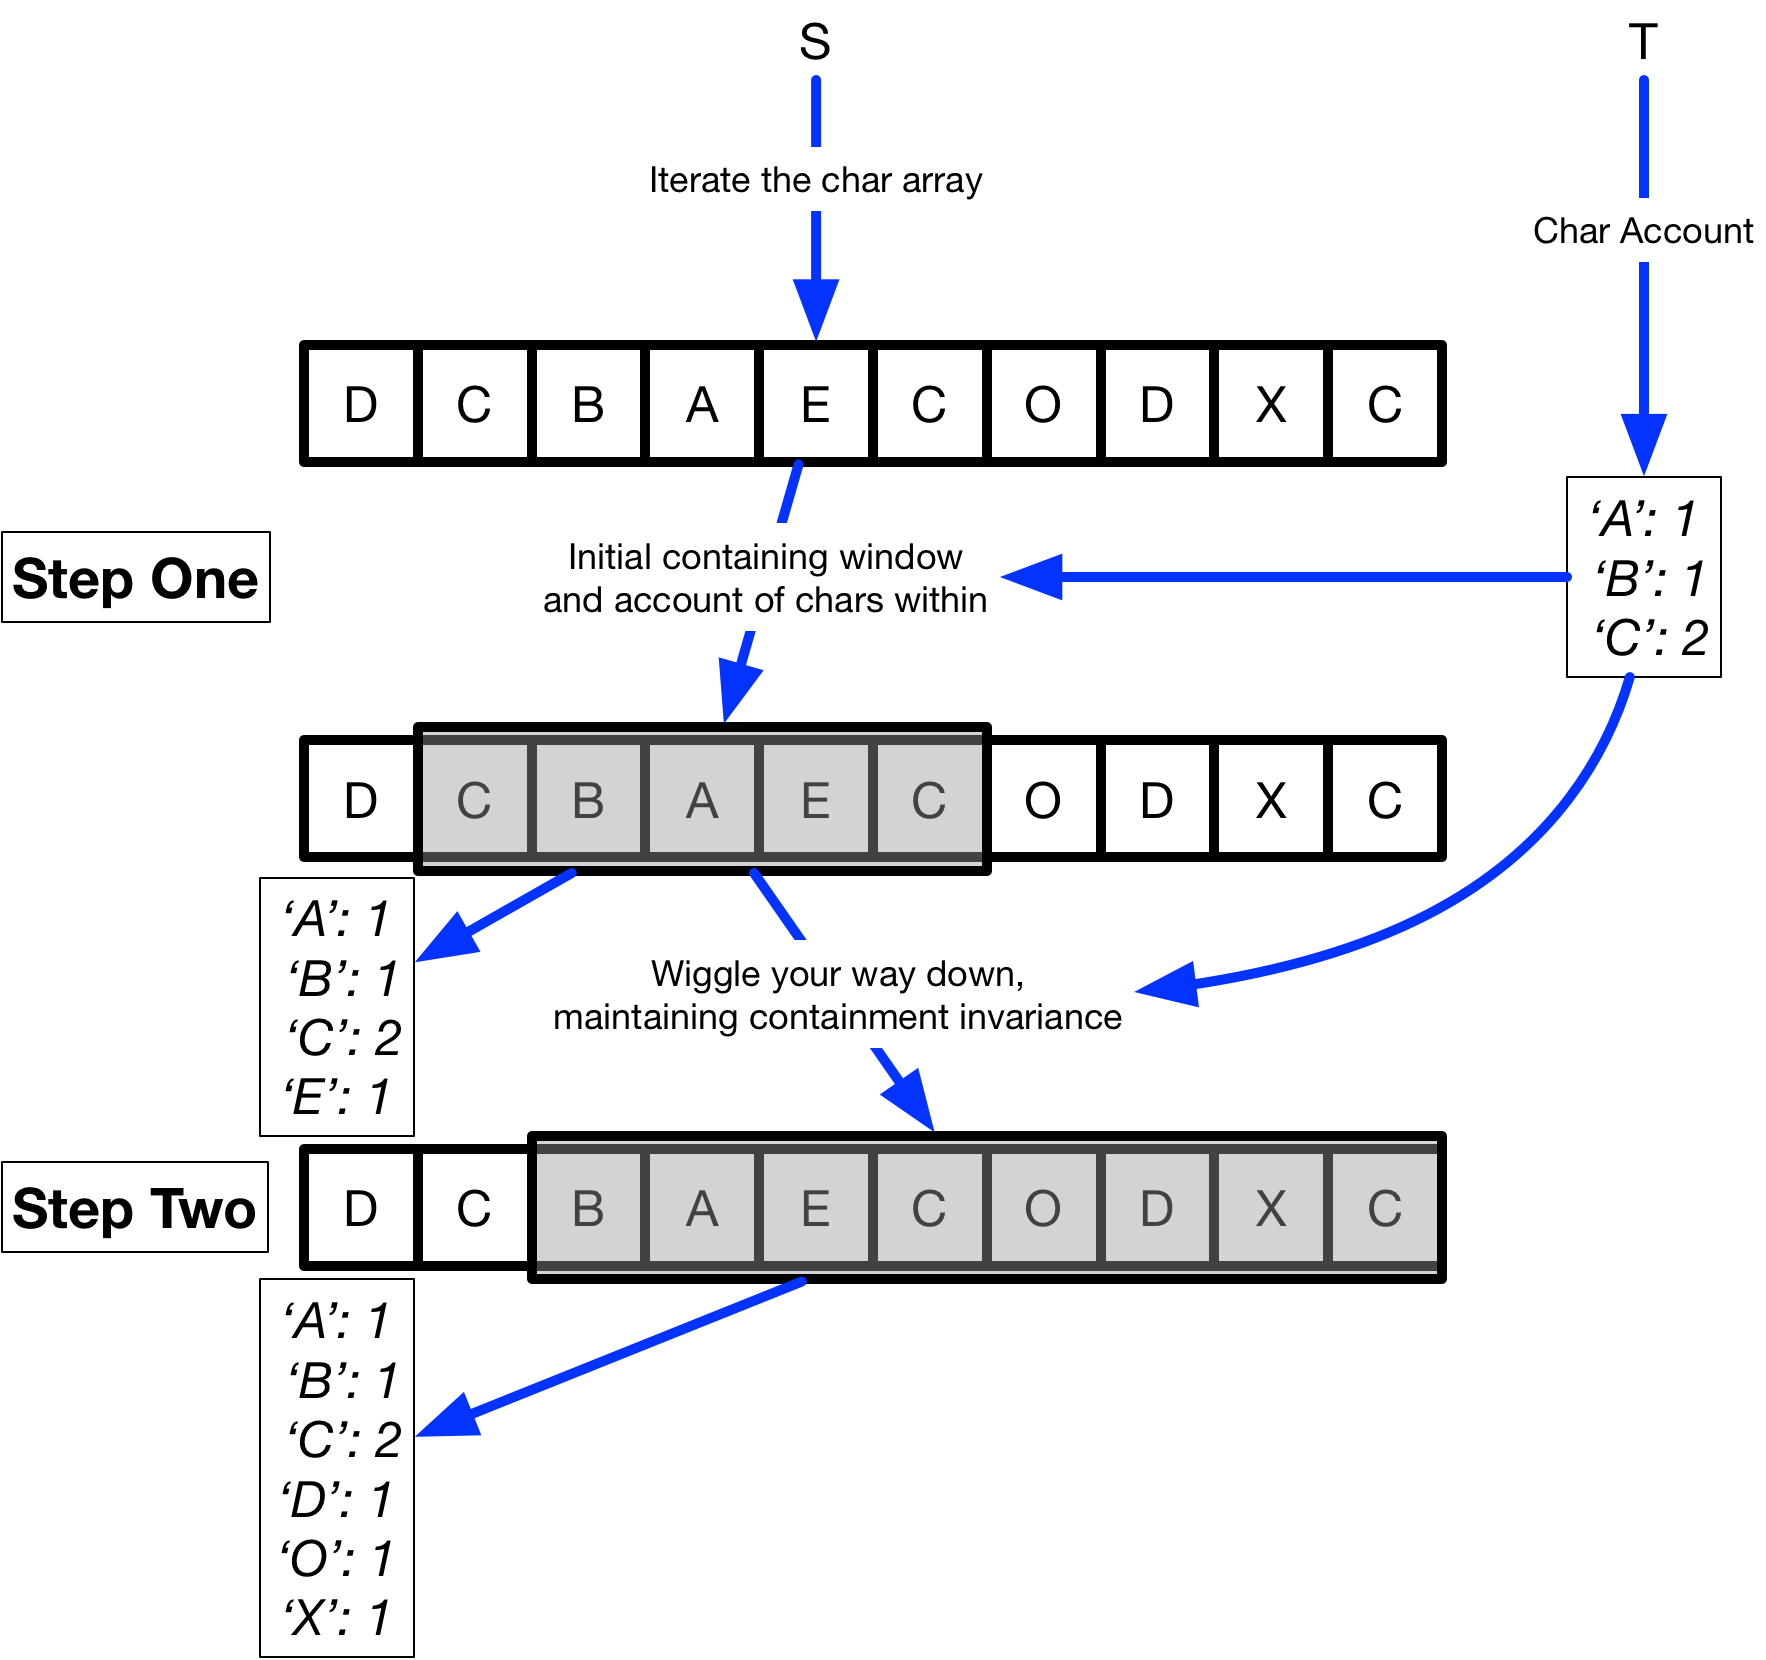
\includegraphics[height=6cm]{case-study/min-window/min-window-algorithm.jpg}
        \caption{A visualization of the algorithm for finding the minimum window containing all
        the characters in the target string \code{T} in source string \code{S}.}
        \label{img:min-window-algorithm.jpg}
    \end{center}
\end{figure}

As one can see my specification of algorithm is high-level and omits many details.
I intend it so that the implementation can have sufficient space for optimization.

\section{Implementations}\label{sec:implementations.min-window}

Both of the problem statement and the optimal algorithm seem pretty straightforward.
One would expect that implementation to be so, too.
Surprisingly, I found that I was wrong after a several failed attempts to implement a clean and
readable solution using languages like \java and \python.
What's more, based on my research on public available implementations on the Internet, almost all
the implementations are so verbose and hard to read (One source may be Leetcode submitted
solutions, visible only after you successfully submit a solution).

So this prompted me to do more research on how to simplify the implementation, how to create
succinct, modular, and readable code.

The subsequent subsections, I'm going to present my approaches of polishing my implementations from
my very first, crude solution to the third solution which is acceptable to me.

As Bruce Lee said ``to the free, creative martial artists, `Absorb what is useful, reject what is
useless, and add what
is essentially your own'.''

To save space, all my implementations adopt the accounting principle `separating the
Revenue and expenditure accounts'.
Namely, I used a map (dictionary in \python) as the intermediate buffer for char surplus.
Populating the buffer is done in one part of the code, and extraction from the buffer is done in
another.
This creates separate grounds for the two major operations and thus greatly promotes modular
designs.

So it's like an asynchronous way of processing.
It stores the character deficit in a map.

Some implementations start with an open set---a set of indexes that are not sufficient to cover
all the character deficit.

But I found that starting with a closed set---a containing window---and then trying
to shorten it is more manageable.

It suffers several issues including verbose, oversize initialization, poor readability, lack
of modular design.

\lstinputlisting[label={lst:MinWindowSubstringVerbose},
caption={An earlier implementation for the `Minimum window' problem.}]
{case-study/min-window/MinWindowSubstringVerbose.java}

For the first time, a technique of sentinel is used to free us from the lengthy
initialization to find a starting point.
The sentinel idea is to prepend the target string \code{T} to the source string \code{S}.
The benefit of doing this is that in the composite string, we readily start with a containing
window---substring from $0$ to \code{len(T)}.
No more lengthy preprocessing to find a containing window within the original source string.

\lstinputlisting[label={lst:MinWindowSubstringSentinel},
caption={A second version of implementation for the `Minimum window' problem.}]
{case-study/min-window/MinWindowSubstring.java}

However, \autoref{lst:MinWindowSubstringSentinel}, a monolithic implementation of a fairly simple
algorithm, is still hard to read.

To fix the issues present in the second version, I implemented the third which is presented in
\autoref{lst:MinWindowSubstringModular}.

A word here: this solution is rarely required for interview.
But this is the ony acceptable version if one is to work in the production environment in a
prestigious company with a sustainable, long-term engineering mission.

\lstinputlisting[label={lst:MinWindowSubstringModular},
caption={A readable version of implementation for the `Minimum window' problem.}]
{case-study/min-window/MinWindowSubstring2018.java}
